\documentclass[paper=a4, fontsize=11pt]{scrartcl}
%\usepackage{sectsty} % Allows for custom section title styling
\usepackage[T1]{fontenc}
\usepackage{fourier} % We're using the Utopia font because it's great.
\usepackage{enumerate} % Allows for custom enumeration types
\usepackage{tikz} % Graphics powered by TikZ!
\usepackage{xcolor} % More colors
\usepackage{listings} % For shell output
\usepackage{nameref} % Reference sections by name, since we're avoiding section numbering

\usetikzlibrary{positioning} % Relative positioning of nodes
\usetikzlibrary{automata} % Handy stuff for state machine diagrams
\usetikzlibrary{shapes.multipart} % Multiline node labels

\tikzstyle{every state}=[fill=orange!30, draw=orange, very thick]
\tikzstyle{free}=[fill=white]
\tikzstyle{link}=[->, draw=cyan, very thick]

\lstdefinestyle{ShellStyle} {
  basicstyle=\small\ttfamily,
  numbers=none,
  frame=tblr,
  columns=fullflexible,
  backgroundcolor=\color{blue!10},
  linewidth=0.9\linewidth,
  xleftmargin=0.1\linewidth
}

%\allsectionsfont{\centering \normalfont\scshape} % Center and semi-cap section titles
\newcommand{\horrule}[1]{\rule{\linewidth}{#1}} % Horizontal rule with weight arg

\title{
  \normalfont \normalsize 
  \textsc{New Mexico Tech} \\ [25pt]
  \horrule{0.5pt} \\[0.4cm]
  \huge CSE 325 --- Lab Project 5 \\ Memory Management \\
  \horrule{2pt} \\[0.5cm]
}

\author{Rob Kelly \& Ian Neal \\ SANIC TEEM}
\date{\normalsize\today}

\begin{document}
\maketitle

%%% INTRODUCTION %%%
The SANIC TEEM Maniac Middle Management Memory Minder (hereafter referred to as \textit{the project}) is a highly-configurable simulated memory manager with a number of different contiguous memory allocation strategies available for use. Specifically, these allocation strategies are as follows:

\begin{description}
  \item[First Fit], which will allocate the suitable\footnote{Here, a ``suitable'' block is a block that is not currently allocated and is large enough to fit the new data.} block that is sequentially first in memory,

  \item[Best Fit], which will allocate the smallest suitable block,

  \item[Worst Fit], which will allocate the largest suitable block, and

  \item[Next Fit], which will allocate the suitable block that is sequentially first in memory \textbf{after the last block allocated,} wrapping around to the start of addressable space upon reaching the end.
\end{description}

Most of the codebase of this project was given as part of the lab assignment. We have implemented the functionality of the project in the following files:

\begin{itemize}
  \item Implementation of all described functionality in \texttt{mymem.c}.

  \item This README, the \LaTeX\hspace{0em} source of which may be found in \texttt{README.tex}.

  \item Build targets for the added files and this README in the \texttt{Makefile}.
\end{itemize}

%%% BUILDING %%%
\section*{Building}
\begin{itemize}
  \item \texttt{make} to build the project normally.

  \item \texttt{make test} to run the provided testing harness.
  \begin{itemize}
    \item \texttt{make test 2> /dev/null} to suppress error output during testing (does not suppress success or failure of tests). By design, the program will print an error message when memory allocation fails for any reason. The provided stress test will sometimes attempt to allocate more memory than will fit in any existing block, which will fail and produce an error as expected. Use this command to prevent stderr from getting spammed.
  \end{itemize}

  \item \texttt{make doc} to build this README. Requires \texttt{pdflatex} and a number of \LaTeX\hspace{0em} packages, all of which are included in the popular \textbf{TeX Live} distribution.

  \item \texttt{make clean} to clean up temporary files, build files, and output.
\end{itemize} 

%%% USAGE %%%
% Taken from memorytests.c:main()
\section*{Usage}
\texttt{mem -test <test> <strategy>}

\begin{itemize}
  \item \texttt{test} is the test to run, which may be \texttt{alloc1}, \texttt{alloc2}, \texttt{alloc3}, \texttt{alloc4}, \texttt{stress}, or \texttt{all} as desired.

  \item \texttt{strategy} is the memory allocation strategy to use, which may be \texttt{first}, \texttt{best}, \texttt{worst}, \texttt{next}, or \texttt{all} as desired. These correspond to the first fit, best fit, worst fit, and next fit strategies (or all of the above) respectively.
\end{itemize}

%%% EXAMPLES %%%
\section*{Examples}
\begin{lstlisting}[style=ShellStyle]
$ ./mem -test all all 2> /dev/null
Running tests...
 1.alloc1              ::pass
 2.alloc2              ::pass
 3.alloc3              ::pass
 4.alloc4              ::pass
 5.stress              ::pass

Test Results:5 tests,5 passed,0 failed.
\end{lstlisting}

%%% DESIGN %%%
\section*{Design \& Implementation}
The implementation of this project relies on a number of globally- and statically-visible structures and variables. While this is not an ideal design pattern by any means, these global variables are an artifact of the code given to our team as part of the assignment and as such have not been eliminated in the interest of compatibility. Specifically, these globally-visible structures are

\begin{itemize}
  \item \texttt{struct memoryList *head}, a pointer to the head of the memory list.
  \item \texttt{struct memoryList *next}, a pointer to most recently allocated block of memory. This is used by the next-fit allocation strategy.
  \item \texttt{void *myMemory}, a pointer to the memory pool from which all memory allocated by our manager is drawn.
  \item \texttt{size\_t mySize}, which holds the size (in bytes) of the memory pool.
\end{itemize}

\subsection*{Memory List}
\begin{figure}[h]
  \centering
  \textit{Before allocation:}\\
  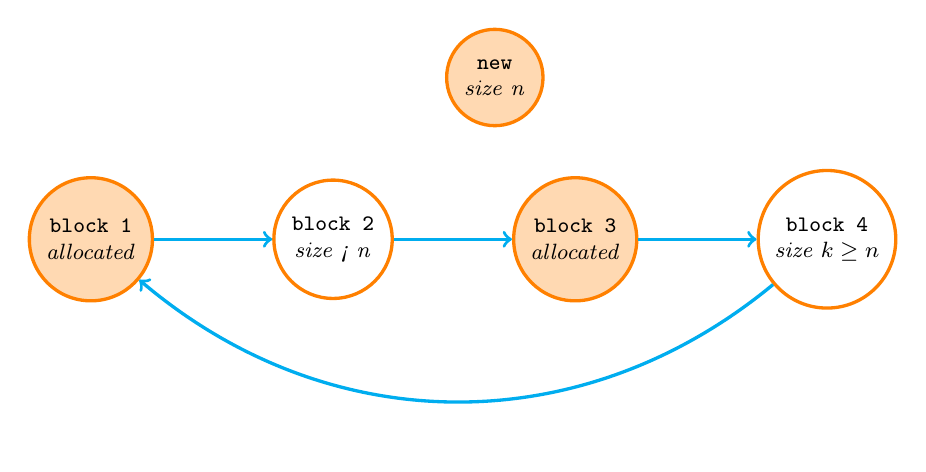
\begin{tikzpicture}[node distance = 1.5cm, auto, every text node part/.style={align=center, font=\footnotesize}]
    \node[state]       (block1)                     {\texttt{block 1}\\\textit{allocated}};
    \node[state, free] (block2) [right = of block1] {\texttt{block 2}\\\textit{size < n}};
    \node[state]       (block3) [right = of block2] {\texttt{block 3}\\\textit{allocated}};
    \node[state, free] (block4) [right = of block3] {\texttt{block 4}\\\textit{size $k \geq n$}};

    \node[state]       (blockn) [above right = of block2] {\texttt{new}\\\textit{size n}};

    \draw[link] (block1) to (block2);
    \draw[link] (block2) to (block3);
    \draw[link] (block3) to (block4);
    \draw[link] (block4) to[bend left=40] (block1);
  \end{tikzpicture}

  \textit{After allocation:}\\
  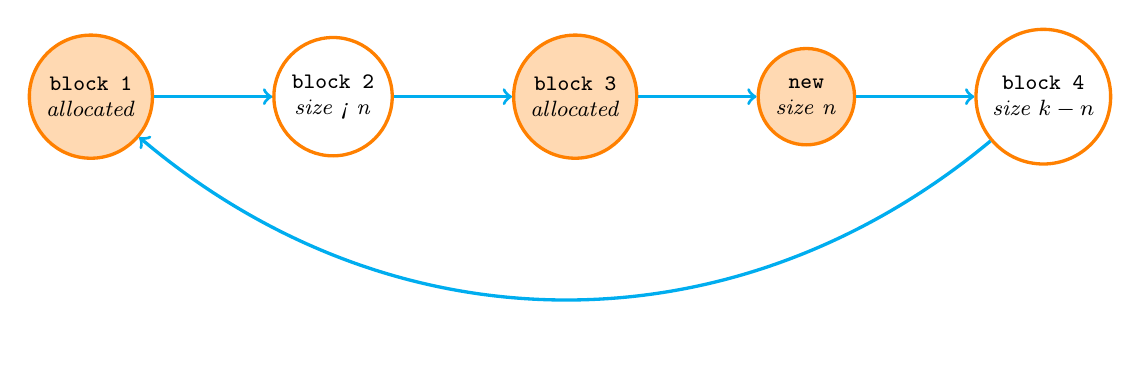
\begin{tikzpicture}[node distance = 1.5cm, auto, every text node part/.style={align=center, font=\footnotesize}]
    \node[state]       (block1)                     {\texttt{block 1}\\\textit{allocated}};
    \node[state, free] (block2) [right = of block1] {\texttt{block 2}\\\textit{size < n}};
    \node[state]       (block3) [right = of block2] {\texttt{block 3}\\\textit{allocated}};
    \node[state]       (blockn) [right = of block3] {\texttt{new}\\\textit{size n}};    
    \node[state, free] (block4) [right = of blockn] {\texttt{block 4}\\\textit{size $k - n$}};


    \draw[link] (block1) to (block2);
    \draw[link] (block2) to (block3);
    \draw[link] (block3) to (blockn);
    \draw[link] (blockn) to (block4);
    \draw[link] (block4) to[bend left=40] (block1);
  \end{tikzpicture}

  \caption{Allocating a block of size $n$.}
  \label{fig:allocation}
\end{figure}

\begin{figure}[h]
  \centering
  \textit{Before freeing block 3:}\\
  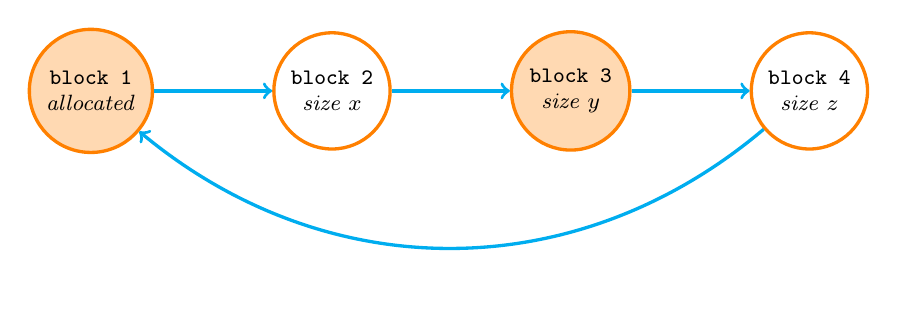
\begin{tikzpicture}[node distance = 1.5cm, auto, every text node part/.style={align=center, font=\footnotesize}]
    \node[state]       (block1)                     {\texttt{block 1}\\\textit{allocated}};
    \node[state, free] (block2) [right = of block1] {\texttt{block 2}\\\textit{size $x$}};
    \node[state]       (block3) [right = of block2] {\texttt{block 3}\\\textit{size $y$}};
    \node[state, free] (block4) [right = of block3] {\texttt{block 4}\\\textit{size $z$}};

    \draw[link] (block1) to (block2);
    \draw[link] (block2) to (block3);
    \draw[link] (block3) to (block4);
    \draw[link] (block4) to[bend left=40] (block1);
  \end{tikzpicture}\\
  \textit{After freeing block 3:}\\
  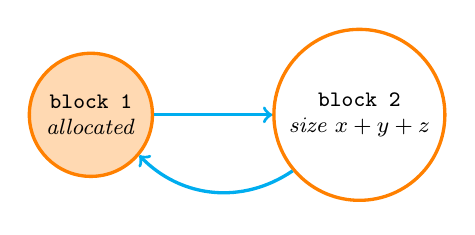
\begin{tikzpicture}[node distance = 1.5cm, auto, every text node part/.style={align=center, font=\footnotesize}]
    \node[state]       (block1)                     {\texttt{block 1}\\\textit{allocated}};
    \node[state, free] (block2) [right = of block1] {\texttt{block 2}\\\textit{size $x+y+z$}};

    \draw[link] (block1) to (block2);
    \draw[link] (block2) to[bend left=40] (block1);
  \end{tikzpicture}

  \caption{Freeing an allocated block.}
  \label{fig:free}
\end{figure}


%%% BUGS %%%
\section*{Known Bugs}
The code for which SANIC TEEM is responsible (contained in \texttt{mymem.c}) has no known bugs or memory leaks. There appear to be memory leaks present in the provided code, which we have made no effort to patch.

\end{document}
